%%%%%%%%%%%%%%%%%%%%%%%%%%%%%%%%%%%%%%%%%%%%%%%%%%%%%%%%%%%%%%%%%%%%%%%%%%%%%%%%
%2345678901234567890123456789012345678901234567890123456789012345678901234567890
%        1         2         3         4         5         6         7         8

\documentclass[letterpaper, 10 pt, conference]{ieeeconf}  % Comment this line out if you need a4paper
%\documentclass[a4paper, 10pt, conference]{ieeeconf}      % Use this line for a4 paper
\IEEEoverridecommandlockouts                              % This command is only needed if 
                                                          % you want to use the \thanks command
\overrideIEEEmargins                                      % Needed to meet printer requirements.
% See the \addtolength command later in the file to balance the column lengths
% on the last page of the document
% The following packages can be found on http:\\www.ctan.org
\usepackage{graphicx} % for pdf, bitmapped graphics files
%\usepackage{mathptmx} % assumes new font selection scheme installed
\usepackage{amsmath} % assumes amsmath package installed
\usepackage{amssymb}  % assumes amsmath package installed
\usepackage{subfigure}
%\usepackage{natbib}
\usepackage{cite}
\usepackage{flushend}
\usepackage[usenames,dvipsnames,svgnames,table]{xcolor}
\usepackage[backref=true,breaklinks=true,hidelinks,colorlinks=false,bookmarks=false,citecolor=green]{hyperref}
\usepackage[acronym]{glossaries}
\usepackage{float}
\usepackage[small,normal,bf,up]{caption}
\usepackage{epstopdf}

\newcommand{\V}[1] {\mathbf{#1}}
\newcommand{\Vx}[0] {\mathbf{x}}
\newcommand{\Vy}[0] {\mathbf{y}}
\newcommand{\Vz}[0] {\mathbf{z}}
\newcommand{\Vu}[0] {\mathbf{u}}
\newcommand{\Vv}[0] {\mathbf{v}}
\newcommand{\Vw}[0] {\mathbf{w}}
\newcommand{\Vm}[0] {\mathbf{m}}

\newcommand{\Vb}[2] {\V{#1}_{#2}}
\newcommand{\Vxb}[1] {\Vx_{#1}}
\newcommand{\Vzb}[1] {\Vz_{#1}}
\newcommand{\Vxp}[1] {\Vx^{#1}}

\newcommand{\Vbp}[3] {\V{#1}_{#2}^{#3}}
\newcommand{\Vxbp}[2] {\Vx_{#1}^{#2}}
\newcommand{\Vzbp}[2] {\Vz_{#1}^{#2}}
\newcommand{\Vubp}[2] {\Vu_{#1}^{#2}}
\newcommand{\Vvbp}[2] {\Vv_{#1}^{#2}}
\newcommand{\Vwbp}[2] {\Vw_{#1}^{#2}}
\newcommand{\VSbp}[2] {\V{\Sigma}_{#1}^{#2}}
\newcommand{\dVxbp}[2] {\dot{\Vxbp{#1}{#2}}}

\newcommand{\pVbp}[4] {{}^{#1}\V{#2}_{#3}^{#4}}
\newcommand{\pVzb}[2] {{}^{#1}\Vz_{#2}}
\newcommand{\pVxbp}[3] {{}^{#1}\Vx_{#2}^{#3}}
\newcommand{\pVvbp}[3] {{}^{#1}\Vv_{#2}^{#3}}
\newcommand{\pVzbp}[3] {{}^{#1}\Vz_{#2}^{#3}}
\newcommand{\ptVzbp}[3] {{}^{#1}\tilde \Vz_{#2}^{#3}}
\newcommand{\ptVzb}[2] {{}^{#1}\tilde\Vz_{#2}}
\newcommand{\tVxp}[1] {\tilde \Vx^{#1}}
\newcommand{\tVxbp}[2] {\tilde \Vx_{#1}^{#2}}
\newcommand{\tVzbp}[2] {\tilde \Vz_{#1}^{#2}}
\newcommand{\tVubp}[2] {\tilde \Vu_{#1}^{#2}}
\newcommand{\tVzb}[1] {\tilde \Vz_{#1}}
\newcommand{\mVxbp}[2] {\bar \Vx_{#1}^{#2}}
\newcommand{\mVmb}[1] {\bar \Vm_{#1}}
\newcommand{\pmVxbp}[3] {{}^{#1}\bar \Vx_{#2}^{#3}}
\newcommand{\bpVp}[4] {{}_{#1}^{#2}\V{#3}^{#4}}

\newcommand{\Sz}[0] {z}
\newcommand{\tSzbp}[2] {\tilde \Sz_{#1}^{#2}}
\newcommand{\ptSzbp}[3] {{}^{#1}\tilde \Sz_{#2}^{#3}}

\newcommand{\sbram}[1] {\left \{ #1 \right .}
\newcommand{\vm}[2] {\bl{\begin{array}{#1} #2 \end{array}}}
\newcommand{\ar}[2] {\begin{array}{#1} #2 \end{array}}
\newcommand{\sbrar}[2] {\sbram{\begin{array}{#1} #2 \end{array}}}
\newcommand{\vmabs}[2] {\abs{\begin{array}{#1} #2 \end{array}}}
\newcommand{\mac}[1] {\left < #1 \right >}

\newcommand{\Cal}[1] {\mathcal{#1}}


\newcommand{\xbp}[2] {x_{#1}^{#2}}
\newcommand{\ybp}[2] {y_{#1}^{#2}}
\newcommand{\thbp}[2] {\theta_{#1}^{#2}}

\newcommand{\bm}[1] {\left \{ #1 \right \}}
\newcommand{\bs}[1] {\left ( #1 \right )}
\newcommand{\bl}[1] {\left [ #1 \right ]}
\newcommand{\bml}[1] {\left \{ #1 \right .}
\newcommand{\bsl}[1] {\left ( #1 \right .}
\newcommand{\bll}[1] {\left [ #1 \right .}
\newcommand{\bmr}[1] {\left . #1 \right \}}
\newcommand{\bsr}[1] {\left . #1 \right )}
\newcommand{\blr}[1] {\left . #1 \right ]}
\newcommand{\mcc}[1] {\left \langle #1 \right \rangle}
\newcommand{\abs}[1] {\left | #1 \right |}
\newcommand{\dabs}[1] {\left \| #1 \right \|}

\newcommand{\p}[1] {\mbox{$ {p} \left ( #1 \right )$ }} % Probability
\newcommand{\li}[1] {l \left ( #1 \right )}
\newcommand{\lio}[1] {l_i^{c} \left ( #1 \right )}
\newcommand{\lia}[1] {l_j^{a} \left ( #1 \right )}
\newcommand{\lid}[1] {l_j^{d} \left ( #1 \right )}
\newcommand{\lir}[1] {l_j^{r} \left ( #1 \right )}
\newcommand{\f}[2] {#1 \left ( #2 \right )}
\newcommand{\Vf}[1] {\mathbf{f} \left ( #1 \right )}
\newcommand{\Vfb}[2] {\mathbf{f}_{#1} \left ( #2 \right )}
\newcommand{\Vfp}[2] {\mathbf{f}^{#1} \left ( #2 \right )}
\newcommand{\Vfbp}[3] {\mathbf{f}_{#1}^{#2} \left ( #3 \right )}
\newcommand{\Vh}[1] {\mathbf{h} \left ( #1 \right )}
\newcommand{\Vhb}[2] {\mathbf{h}_{#1} \left ( #2 \right )}
\newcommand{\Vhp}[2] {\mathbf{h}^{#1} \left ( #2 \right )}
\newcommand{\pVhp}[3] {{}^{#1}\mathbf{h}^{#2} \left ( #3 \right )}
\newcommand{\Vhbp}[3] {\mathbf{h}_{#1}^{#2} \left ( #3 \right )}
\newcommand{\pVgp}[3] {{}^{#1}\mathbf{g}^{#2} \left ( #3 \right )}

% general global definitions
\newcommand{\Def}{\ {\buildrel \triangle\over =}\ }
\newcommand{\beq} {\begin{equation}}
\newcommand{\eeq} {\end{equation}}
\newcommand{\beqn} {\begin{eqnarray}}
\newcommand{\eeqn} {\end{eqnarray}}
\newcommand{\E}[1] {\mbox{$ {\rm E} \{ #1 \}$ }}
\newcommand{\Es}[2] {\mbox{$ {\rm E}^{#1} \{ #2 \}$ }}
\newcommand{\Set}[1] {\mbox{$ \{ #1 \} $ }}
\newcommand{\Cali}[2] {\mbox{$ {\cal #1 }_{#2} $}}
\newcommand{\PR}[1]  {\mbox{$ P(#1) $}}
\newcommand{\Pri}[2]  {\mbox{$ P_{#1}(#2) $}}
\newcommand{\PRi}[2]  {\mbox{$ P_{#1}(#2) $}}
\newcommand{\Pris}[3]  {\mbox{$ P_{#1}^{#2}(#3) $}}
\newcommand{\like}[1]  {\mbox{$ \Lambda(\bf #1) $}}
\newcommand{\likei}[2]  {\mbox{$ \Lambda_{#2}(\bf #1) $}}
\newcommand{\LL}[1]  {\mbox{$ l(#1) $}} % loglikelihood
\newcommand{\LLi}[2]  {\mbox{$ l_{#1}(#2) $}} %loglikelihood
\newcommand{\EN}[1]  {\mbox{$ H(#1) $}} % entropy
\newcommand{\ENi}[2]  {\mbox{$ H_{#1}(#2) $}} % entropy
\newcommand{\mEN}[1]  {\mbox{$ \overline{H}(#1) $}} % mean entropy
\newcommand{\MI}[1]  {\mbox{$ I(#1) $}}  %mutual information
\newcommand{\est}[1]  {\mbox{$\hat{\bf #1}$}}
\newcommand{\estk}[2]  {\mbox{$\hat{\bf #1}(#2)$}}
\newcommand{\esti}[2]  {\mbox{$\hat{\bf #1}_{#2}$}}
\newcommand{\D}[1]    {\mbox{${\rm d} {#1}$}}
\newcommand{\mean}[1] {\mbox{$\overline{ #1}$}}
\newcommand{\Det}[1] {\mbox{$\mid {#1} \mid $}}
\newcommand{\One}      {\mbox{${\bf 1}$}}
\newcommand{\Zero}      {\mbox{${\bf 0}$}}
\newcommand{\grad}[1] {\mbox{${\bf\nabla} #1$}}
\newcommand{\J}[3] {\mbox{${\bf\nabla}{\bf #1}_{\bf #2}(#3)$}}
\newcommand{\Jt}[3] {\mbox{${\bf\nabla}^T{\bf #1}_{\bf #2}(#3)$}}
\newcommand{\pdf}{{\it pdf\ }}
\newcommand{\dxt}[2]  {\mbox{$\dot{\bf #1}( #2)$}}
% defining different types of vectors
% first those with no time subscripts
\newcommand{\Vt}[1] {\mbox{${\bf #1}^T$}}
\newcommand{\Vin}[1] {\mbox{${\bf #1}^{-1}$}}
\newcommand{\Vgin}[1] {\mbox{${\bf #1}^{\dagger}$}}
\newcommand{\Vi}[2] {\mbox{${\bf #1}_{#2}$}}
\newcommand{\Vs}[2] {\mbox{${\bf #1}^{#2}$}}
\newcommand{\Vis}[3] {\mbox{${\bf #1}_{#2}^{#3}$}}
\newcommand{\Vit}[2] {\mbox{${\bf #1}_{#2}^T$}}
\newcommand{\Vini}[2] {\mbox{${\bf #1}_{#2}^{-1}$}}
\newcommand{\Vgini}[2] {\mbox{${\bf #1}^{\dagger}$}}
\newcommand{\tV}[1] {\mbox{$\tilde{\bf #1}$}}
\newcommand{\tVi}[2] {\mbox{$\tilde{\bf #1}_{#2}$}}
\newcommand{\tVini}[2] {\mbox{$\tilde{\bf #1}_{#2}^{-1}$}}
\newcommand{\tick}  {\mbox{$\delta t$}}

% next those with time subscript k (very common)
\newcommand{\Vk}[1] {\mbox{${\bf #1}(k)$}}
\newcommand{\Vkt}[1] {\mbox{${\bf #1}^T(k)$}}
\newcommand{\Vkin}[1] {\mbox{${\bf #1}^{-1}(k)$}}
\newcommand{\Vkgin}[1] {\mbox{${\bf #1}^{\dagger}(k)$}}
\newcommand{\Vki}[2] {\mbox{${\bf #1}_{#2}(k)$}}
\newcommand{\Vks}[2] {\mbox{${\bf #1}^{#2}(k)$}}
\newcommand{\Vkis}[3] {\mbox{${\bf #1}_{#2}^{#3}(k)$}}
\newcommand{\Vkit}[2] {\mbox{${\bf #1}_{#2}^T(k)$}}
\newcommand{\Vkini}[2] {\mbox{${\bf #1}_{#2}^{-1}(k)$}}
\newcommand{\Vkgini}[2] {\mbox{${\bf #1}^{\dagger}_{#2}(k)$}}
\newcommand{\tVk}[1] {\mbox{$\tilde{\bf #1}(k)$}}
\newcommand{\tVki}[2] {\mbox{$\tilde{\bf #1}_{#2}(k)$}}

% now those with general purpose time subscripts
%\newcommand{\Vec}[2] {\mbox{${\bf #1}(#2)$}}
\newcommand{\Vect}[2] {\mbox{${\bf #1}^T(#2)$}}
\newcommand{\Vecin}[2] {\mbox{${\bf #1}^{-1}(#2)$}}
\newcommand{\Veci}[3] {\mbox{${\bf #1}_{#2}(#3)$}}
\newcommand{\Vecs}[3] {\mbox{${\bf #1}^{#2}(#3)$}}
\newcommand{\Vecit}[3] {\mbox{${\bf #1}_{#2}^T(#3)$}}
\newcommand{\Vecini}[3] {\mbox{${\bf #1}_{#2}^{-1}(#3)$}}
\newcommand{\Vecgin}[2] {\mbox{${\bf #1}^{\dagger}(#2)$}}
\newcommand{\Vecgini}[3] {\mbox{${\bf #1}^{\dagger}_{#2}(#3)$}}

% special symbols used very commonly
% state estimates of different sorts
\newcommand{\x}[2] {\mbox{$\hat{\bf x}( #1 \mid #2)$}}
\newcommand{\xj}[3] {\mbox{$\hat{\bf x}_{#1}( #2 \mid #3)$}}
\newcommand{\tx}[2] {\mbox{$\tilde{\bf x}( #1 \mid #2 )$}}
\newcommand{\txt}[2] {\mbox{$\tilde{\bf x}^T( #1 \mid #2 )$}}
\newcommand{\txi}[3] {\mbox{$\tilde{\bf x}_{#1}( #2 \mid #3 )$}}
\newcommand{\txit}[3] {\mbox{$\tilde{\bf x}^T_{#1}( #2 \mid #3 )$}}
\newcommand{\z}[2] {\mbox{$\hat{\bf z}( #1 \mid #2)$}}
\newcommand{\tz}[2] {\mbox{$\tilde{\bf z}( #1 \mid #2)$}}
\newcommand{\tzt}[2] {\mbox{$\tilde{\bf z}^T( #1 \mid #2)$}}
\newcommand{\zi}[3] {\mbox{$\hat{\bf z}_{#1}( #2 \mid #3)$}}
\newcommand{\di}[3] {\mbox{$\hat{\bf \delta}_{#1}( #2 \mid #3)$}}

% variances of different sorts
\newcommand{\var}[2] {\mbox{${\bf P}( #1 \mid #2)$}}
\newcommand{\varin}[2] {\mbox{${\bf P}^{-1}( #1 \mid #2)$}}
\newcommand{\tvar}[2] {\mbox{$\tilde{\bf P}( #1 \mid #2)$}}
\newcommand{\tvarin}[2] {\mbox{$\tilde{\bf P}^{-1}( #1 \mid #2)$}}
\newcommand{\vari}[3] {\mbox{${\bf P}_{#1}( #2 \mid #3)$}}
\newcommand{\varit}[3] {\mbox{${\bf P}^T_{#1}( #2 \mid #3)$}}
\newcommand{\varini}[3] {\mbox{${\bf P}^{-1}_{#1}( #2 \mid #3)$}}
\newcommand{\tvari}[3] {\mbox{$\tilde{\bf P}_{#1}( #2 \mid #3)$}}
\newcommand{\tvarini}[3] {\mbox{$\tilde{\bf P}^{-1}_{#1}( #2 \mid #3)$}}

% information states and variances
\newcommand{\y}[2] {\mbox{$\hat{\bf y}( #1 \mid #2)$}}
\newcommand{\ty}[2] {\mbox{$\tilde{\bf y}( #1 \mid #2)$}}
\newcommand{\yi}[3] {\mbox{$\hat{\bf y}_{#1}( #2 \mid #3)$}}
\newcommand{\tyi}[3] {\mbox{$\tilde{\bf y}_{#1}( #2 \mid #3)$}}
\newcommand{\Y}[2] {\mbox{${\bf Y}( #1 \mid #2)$}}
\newcommand{\Yin}[2] {\mbox{${\bf Y}^{-1}( #1 \mid #2)$}}
\newcommand{\tY}[2] {\mbox{$\tilde{\bf Y}( #1 \mid #2)$}}
\newcommand{\Yi}[3] {\mbox{${\bf Y}_{#1}( #2 \mid #3)$}}
\newcommand{\Yini}[3] {\mbox{${\bf Y}_{#1}^{-1}( #2 \mid #3)$}}
\newcommand{\tYi}[3] {\mbox{$\tilde{\bf Y}_{#1}( #2 \mid #3)$}}
\newcommand{\info}[1] {\mbox{${\bf i}( #1)$}}
\newcommand{\Info}[1] {\mbox{${\bf I}( #1)$}}
\newcommand{\infoi}[2] {\mbox{${\bf i}_{#1}( #2)$}}
\newcommand{\infois}[3] {\mbox{${\bf i}_{#1}^{#2}(#3)$}}
\newcommand{\Infoi}[2] {\mbox{${\bf I}_{#1}( #2)$}}
\newcommand{\tInfoi}[2] {\mbox{$\tilde{\bf I}_{#1}( #2)$}}
\newcommand{\Infoin}[1] {\mbox{${\bf I}^{\dagger}( #1)$}}
\newcommand{\Infoini}[2] {\mbox{${\bf I}^{\dagger}_{#1}( #2)$}}
\newcommand{\Prop}[2] {\mbox{${\bf L}( #1 \mid #2)$}}
\newcommand{\Propi}[3] {\mbox{${\bf L}_{#1}( #2 \mid #3)$}}
\newcommand{\Z}[2] {\mbox{${\cal Z}^{#1}_{#2}$}}

% spurious ones
\newcommand{\maybe}{\ {\buildrel ?\over =}\ } %chapter 4
\newcommand{\svd} {\mbox{$\dagger$}} % chapter 4
\newcommand{\dnoise} {\mbox{$\delta d$}} % chapter 6 and 7
\newcommand{\unoise} {\mbox{$\delta u$}} % chapter 6
\newcommand{\ns}[1] {\mbox{$ #1$}} % chapter 6
\newcommand{\vs} {\vspace{0.17in}}
\newcommand{\svs} {\vspace{0.17cm}}
\newcommand{\vsf} {\vspace{0.4in}}
\newcommand{\vsff} {\vspace{1in}}
\newcommand{\veqns} {\vspace{-0.15in}}
\newcommand{\veqn} {\vspace{-0.12in}}
\newcommand{\sveqn} {\vspace{-0.06in}}
\newcommand{\bc}{\begin{center}}
\newcommand{\ec}{\end{center}}
\newcommand{\bi}{\begin{itemize}}
\newcommand{\ei}{\end{itemize}}
\newcommand{\be}{\begin{enumerate}}
\newcommand{\ee}{\end{enumerate}}
\newcommand{\Quote}{\parbox[t]{12.5cm}}
%\newtheorem{example}{Example}

\newcommand{\myline} {\rule[1mm]{100mm}{1mm}}
\newcommand{\egend} {\rule[1mm]{125mm}{1mm}}
\newcommand{\egbegin} {\rule[1mm]{100mm}{1mm}}
\newcommand{\Stitle}[1]{\centering{ {\huge{ {\bf #1} }}}}

\title{\LARGE \bf
Non-Field-Of-View Indoor Sound Source Localization based on Reflection and Diffraction}
\author{Kuya Takami$^{*1}$, Tomonari Furukawa$^{1,2}$ Makoto Kumon$^{3}$ and Lin Chi Mak$^{4}$% <-this % stops a space
\thanks{*Corresponding author}%
%\thanks{**This work was not supported by any organization}% <-this % stops a space
\thanks{$^{1}$Department of Mechanical Engineering, Virginia Polytechnic Institute and State University, USA
        {\tt\small \{kuya, tomonari\}@vt.edu}}
\thanks{$^{2}$Center for Autonomous Systems, University of Technology, Sydney ,NSW, Australia
        {\tt\small}}      
\thanks{$^{3}$Department of Mechanical System Engineering, Kumamoto University, Kumamoto, Japan
        {\tt\small makoto@gpo.kumamoto-u.ac.jp}}
\thanks{$^{4}$AP Photonics Limited,Science Park, Hong Kong
        {\tt\small maklinchi@gmail.com}}
        }
       
\newacronym{2d}{2D}{two-dimensional}
\newacronym{3d}{3D}{three-dimensional}
\newacronym{adc}{ADC}{analogue-to-digital conversion}
\newacronym{imu}{IMU}{inertial measurement unit}
\newacronym{gps}{GPS}{global positioning system}
\newacronym{los}{LOS}{line-of-sight}
\newacronym{nlos}{NLOS}{non-line-of-sight}
\newacronym{mic}{mic}{microphone}
\newacronym{pc}{PC}{personal computer}
\newacronym{tdoa}{TDOA}{time-difference-of-arrival}
\newacronym{toa}{TOA}{time-of-arrival}
\newacronym{USB}{USB}{universal serial bus}

\newacronym{rss}{RSS}{received signal strength}
\newacronym{wgn}{WGN}{white Gaussian noise}
\newacronym{rms}{RMS}{root mean squared}
\newacronym{FPGA}{FPGA}{field programmable gate array}
\newacronym{nfov}{NFOV}{non-field-of-view}
\newacronym{fov}{FOV}{field-of-view}
\newacronym{rbe}{RBE}{recursive Bayesian estimation}
\newacronym{rf}{RF}{radio-frequency}
\newacronym{wsn}{WSN}{wireless sensor network}
\newacronym{ild}{ILD}{interaural level difference}
\newacronym{cmos}{CMOS}{complementary metal-oxide-semiconductor}
\newacronym{ccd}{CCD}{charge-coupled device}
\newacronym{IO}{I/O}{input/output}
\newacronym{sar}{SAR}{search-and-rescue}
\newacronym{dslr}{DSLR}{digital  single-lens reflex}
\newacronym{daq}{DAQ}{data acquisition}
\newacronym{slam}{SLAM}{simultaneous localization and mapping}
\newacronym{ipd}{IPD}{interaural phase difference}
\newacronym{kl}{KL}{Kullback-Leibler}
\newacronym{itd}{ITD}{interaural Time difference}
\newacronym{fft}{FFT}{fast Fourier transform}
\newacronym{SNR}{SNR}{signal-to-noise ratio}

\newglossaryentry{k}{
name=$k$,
description={time index},
sort=k
}
\newglossaryentry{st}{
name=$\Vxbp{k}{t}$,
description={$\in \Cal{X}^t$ state of the target at time step $k$},
sort=state
}
\newglossaryentry{inst}{
name=$\tilde{\bs{}}$,
description={an instance of $\bs{}$},
sort=inst}

\begin{document}
\maketitle
\thispagestyle{empty}
\pagestyle{empty}
%%%%%%%%%%%%%%%%%%%%%%%%%%%%%%%%%%%%%%%%%%%%%%%%%%%%%%%%%%%%%%%%%%%%%%%%%%%%%%%%
\begin{abstract}
This paper presents a new acoustic approach to locate a mobile target outside the \gls{fov}, or the \gls{nfov} of an optical sensor, based on the reflection and diffraction signals. In this approach, a sensor platform determines a reflection \gls{tdoa} and frequency dependent diffraction to two distinct observation likelihoods from a single target's sound. The fusion of these likelihoods, a joint acoustic observation likelihood, estimate the \gls{nfov} target probabilistically within the \gls{rbe} framework. The approach was formulated and derived mathematically. Through parametric studies in simulation, the potential of the proposed approach for practical implementation has been demonstrated by the successful localization of the sound source. Finally, a preliminary validation of sound separation was performed in a controlled experimental environment showing the difference between diffraction alone and combination of diffraction and reflection signals.
\end{abstract}
%%%%%%%%%%%%%%%%%%%%%%%%%%%%%%%%%%%%%%%%%%%%%%%%%%%%%%%%%%%%%%%%%%%%%%%%%%%%%%%%
\section{Introduction}
Sound localization and speech recognition are increased demand for variety of robotic applications where autonomous mobile robots are operating in human and natural settings. Complex environment, such as an indoor setting, produces difficulties to the target localization and tracking, or mobile target estimation. However, it has a variety of applications such as home security, home health care, and urban search-and-rescue with the limitation constrained by the complexity of the indoor structure~\cite{priyantha2005mobile,Khoury2009,argentieri2014survey}. Indoor structures make estimation problems challenging as they can introduce largely unobservable regions when an optical sensor like a camera is deployed.  This is because optical sensors' \acrfull{fov} is determined by the \gls{los} and range of the optical sensor, which is small in highly constrained environments. However, in human settings, humans have the capability to perform searching and finding the target person who is not in the \gls{fov} by communicating with the person and estimating the location. In such a case, target estimation is mostly performed not through vision but audition. 

Sound source localization traditionally focused strictly on \gls{los} conditions based on both time and frequency domain approach. The most common approach utilizes the \acrfull{toa}/\acrfull{tdoa} information of acoustic signals~\cite{hu2011simultaneous,ward2003particle,Mak2009}. Recent work has tackled \acrfull{nfov} target estimation with use of the reflection signal within a known environment. Narang et al.~\cite{narang2014auditory} detected reflected sound effectively using a combination of an image model and dynamic environment map to assists in robot navigation. This approach identifies and estimate the direction of the sound source. However, it does not estimate the target position in \gls{nfov} and does not integrate the vision information for localization. Even et al.~\cite{even2014audio} localized the sound source by a ray tracing method based on the reflected signal arrival directions. However, their approach resulted in \gls{nfov} estimation with meter order accuracy and some inconsistent variations between trails.
%
%  The former \gls{toa}/\gls{tdoa} based acoustic techniques, however, have not achieved true \gls{nfov} target estimation, and latter approach does not fully utilize first arrival diffraction signal information. Furthermore, the majority of sound localization challenges have been focused on the direction of sound rather than its position due to the complexity of sound wave propagation~\cite{tamai2005three,sva12}.
%Recent work for \acrfull{nfov} mobile target estimation has been tackled in three different ways. The first approach deploys target mounted \gls{rf} transmitters and fixed receivers in the environment.  In one arrangement, \gls{rf} receivers form a \gls{wsn}, and numerical techniques are used to localize a \gls{nfov} target by processing information of received signals such as signal intensity~\cite{Dai2012,Guvenc2009}. An improved arrangement with minimal infrastructure uses ``fingerprints''~\cite{Bahl2000,lad04}. There is a unique fingerprint at each location in a static environment.  A target can thus be localized by feature-matching the fingerprints.  Whilst this arrangement can achieve higher accuracy, the critical problem inherent in the \gls{rf} based approach is its applicability only to near-\gls{nfov} target estimation~\cite{priyantha2005mobile,Seow2008}. 

For a numerical technique, existing approaches enhance \gls{nfov} target estimation by including a sensor with a limited \gls{fov}, such as an optical sensor. Mauler~\cite{mau03} stated the \gls{nfov} estimation problem mathematically, and Furukawa,~{\it et al.}~\cite{fur06,fur12} developed a generalized numerical solution.  In this technique, the event of ``no detection'' is converted into an observation likelihood and utilized to positively update probabilistic belief on the target. This belief is dynamically maintained by the \gls{rbe}.  The technique, however, has been found to fail in target estimation unless the target is re-discovered within a short period after being lost. Takami et al.~\cite{takami2015ar} incorporated an acoustic sensor to maintain belief with no optical detection with more reliability. Nevertheless, the technique performed poorly unless the target re-entered the optical \gls{fov} since the acoustic sensing is only conducted in an assistive capacity. Extending Kumon's approach, Takami, {\it et al.}~\cite{takami2015fsr} focused more towards complex indoor environment using \gls{ild} {\it a priori} fixed microphone array knowledge. However, this approach requires prior data collection and can not be applied to the dynamic sensor platforms.

This paper presents a new acoustic approach to estimate a \gls{nfov} mobile target using sound wave physical properties, reflection, and diffraction. In the approach, sound source reflection and diffraction signal \gls{tdoa} and frequency dependent property construct two distinct observation likelihoods from target sound. The fusion of these likelihoods, a joint acoustic observation likelihood, is derived to perform the target estimation. The location of the \gls{nfov} target is finally estimated within the recursive Bayesian estimation framework. This process of target estimation was derived mathematically. Following the formulation, the proposed approach was tested through simulation and parametrically studied under multiple conditions. Finally, an experimental environment was constructed to identify the distinct differences between a diffraction signal alone and combination of diffraction and reflection signals.

\section{\acrfull{nfov}}
\subsection{Auditory Recursive Bayesian Estimation}
The proposed approach is mathematically described as follows. Let the state of the robot $s$ at time step $k$ be $\mVxbp{k}{s} \in \Cal{X}^s$. Consider a target $t$, the state is given by $\Vxbp{k}{t} \in \Cal{X}^t$, and a sequence of observations of the target $t$ by the robot $s$ from time step $1$ to time step $k$ given by $\ptVzbp{s}{1:k}{t} \equiv \bm{\ptVzbp{s}{\kappa}{t}|\forall \kappa \in \bm{1,...,k}}$. The \gls{rbe} represents belief on the target in the form of a probability density function and iteratively updates the belief in time and observation.  Let the belief given a sequence of observations and the robot state at time step ${k-1}$ be  $\p{\Vxbp{k-1}{t}|\ptVzbp{s}{1:k-1}{t},\mVxbp{k-1}{s}}$. Chapman-Kolmogrov equation updates the prior belief in time, or predicts the belief at time step $k$, by the probabilistic motion model $\p{\Vxbp{k}{t}|\Vxbp{k-1}{t},\mVxbp{k-1}{s}}$: 
\begin{multline}\label{eq:predictT}
\p{\Vxbp{k}{t}|\ptVzbp{s}{1:k-1}{t},\mVxbp{k-1}{s}} =\\ \int_{\Cal{X}^t} \p{\Vxbp{k}{t}|\Vxbp{k-1}{t},\mVxbp{k-1}{s}} \\  \p{\Vxbp{k-1}{t}|\ptVzbp{s}{1:k-1}{t},\mVxbp{k-1}{s}} d\Vxbp{k-1}{t}.
\end{multline}
Note that the motion model is $\p{\Vxbp{k}{t}|\Vxbp{k-1}{t}}$ if the target is not reactive to the robot.  The observation update, or the correction process, is performed using the Bayes theorem.  The target belief is corrected using the new observation $\ptVzbp{s}{k}{t}$ as
\begin{eqnarray}\label{eq:correctT}
\p{\Vxbp{k}{t}|\ptVzbp{s}{1:k}{t},\mVxbp{k}{s}} =  \frac{\f{q}{\Vxbp{k}{t}|\ptVzbp{s}{1:k}{t},\mVxbp{k-1:k}{s}}} {\int_{\Cal{X}^t}
    \f{q}{\Vxbp{k}{t}|\ptVzbp{s}{1:k}{t},\mVxbp{k-1:k}{s}} d\Vxbp{k}{t}},
\end{eqnarray}
where $\f{q}{\cdot} = {\li{\Vxbp{k}{t}|\ptVzbp{s}{k}{t}} \p{\Vxbp{k}{t}|\ptVzbp{s}{1:k-1}{t},\mVxbp{k-1}{s}}}$ and $\li{\Vxbp{k}{t}|\ptVzbp{s}{k}{t},\mVxbp{k}{s}}$ represents the observation likelihood of $\Vxbp{k}{t}$ given $\ptVzbp{s}{k}{t}$, $\mVxbp{k}{s}$.  

\begin{eqnarray}\label{eq:joint}
\li{\Vxbp{k}{t}|\ptVzbp{s}{k}{t},\mVxbp{k}{s}} =  \prod_j \lia{\Vxbp{k}{t}|\ptVzbp{s}{k}{t},\mVxbp{k}{s}} 
\end{eqnarray}
where $\lia{\cdot}$ are the likelihoods of $j$th acoustic sensor.

%%%%%%%%%%% begin figure %%%%%%%%%%%%%%%%%%%
\begin{figure}[h]
    {\centering
        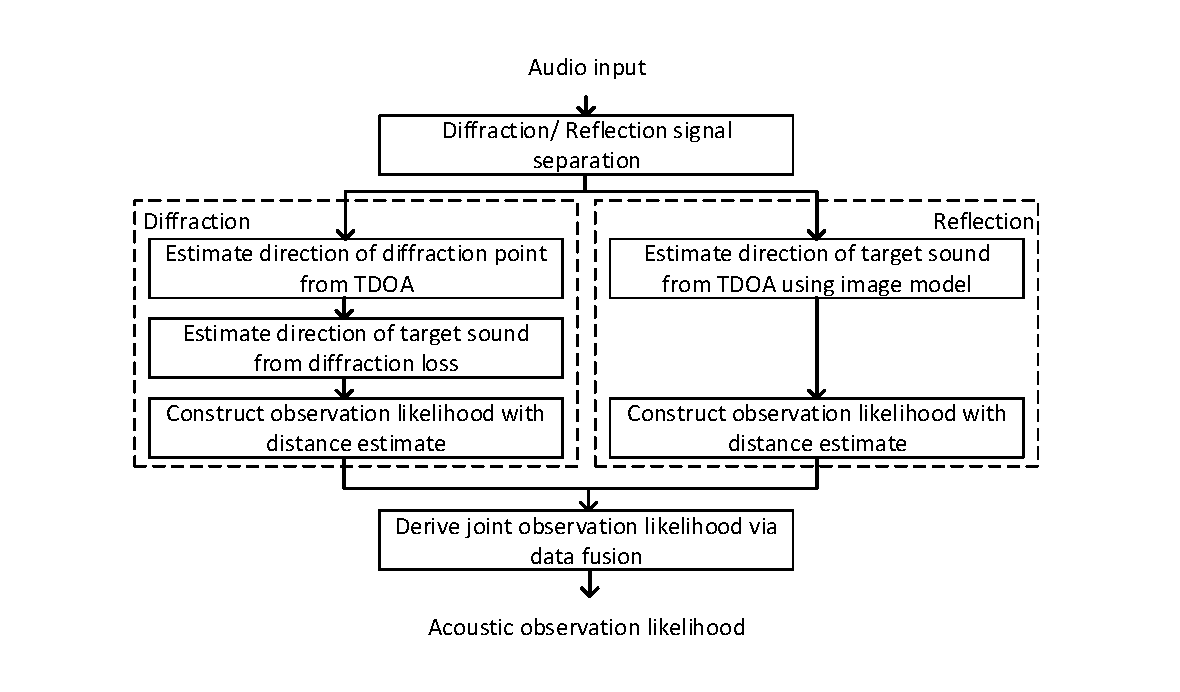
\includegraphics[trim =20mm 15mm 20mm 5mm,width=\columnwidth]{Figures/approach.pdf}
%         \includesvg{Figures/approach}
    }
    \caption{\footnotesize {Construction of auditory NFOV target likelihood} }
    \label{fig:auditory_procedure}
\end{figure}
%%%%%%%%%%%%%%%% end figure %%%%%%%%%%%%%%%%%%%
\subsection{Construction of Auditory NFOV Target Observation Likelihood}
Figure~\ref{fig:auditory_procedure} shows the overview of the approach proposed for constructing a \gls{nfov} target observation likelihood using auditory sensors. The proposed approach extracts the first-arrival diffraction and reflection signals by taking the wave propagation physical properties into account. The approach begins with obtaining a time-domain signal of a relatively impulsive sound at each microphone. In each curve, notable peaks are then extracted as a candidate for first-arrival diffraction and reflection signals. When each candidate signal is described in the frequency domain, the first-arrival diffraction and reflection signals can be identified since they are the first signals that are correlated in the low-frequency range. The diffraction signal is then used to identify the so-called diffraction point by deriving the \gls{tdoa} for each pair of microphones and further estimate the direction of target sound beyond the diffraction point from the loss of sound energy through diffraction, or the diffraction loss. An observation likelihood is eventually constructed by additionally estimating the distance from the sound magnitude and features. The reflection signal estimates the target direction directly from the \gls{tdoa} by mirroring and creating a virtual target.  It also creates an observation likelihood with distance estimate by considering the sound magnitude and characteristics and environmental properties. A joint observation likelihood is finally created by the fusion of the diffraction and reflection observation likelihoods.  

\begin{figure}[ht]
    \centering
    \subfigure[Acoustic signals from NFOV target]{
        \centering
        \label{fig:NFOV_acoustic}
        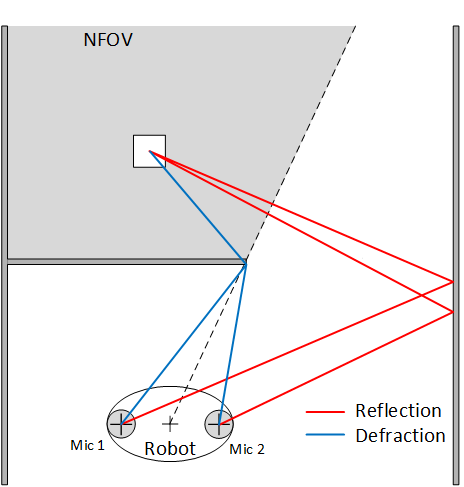
\includegraphics[width=0.7\columnwidth]{Figures/Reflection_diffraction.png}
    }
    \subfigure[Diffracted and reflected signals]{
        \centering
        \label{fig:sound_extraction}
        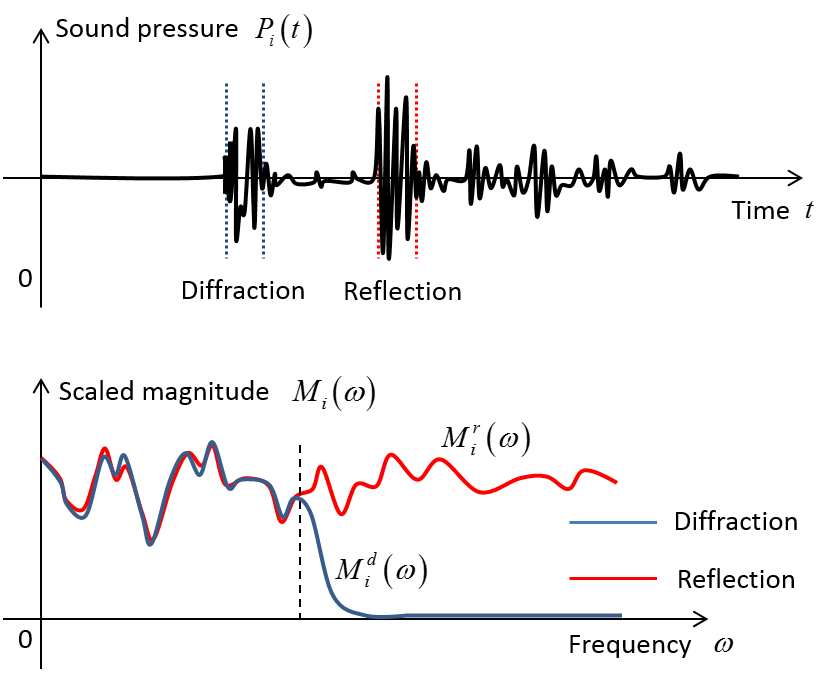
\includegraphics[width=0.7\columnwidth]{Figures/sound_extraction.png}
    }
    \caption{Auditory NFOV target observation}
    \label{fig:auditory_approach}
\end{figure}

The proposed approach infers the location of the sound target using both the first-arrival diffracted and reflected sound signals.  The next subsection describes the extraction of the first-arrival diffraction and reflection signals, followed by the target estimation using the diffracted and reflected signals in the subsequent two subsections.  The final goal of this project is to develop a probabilistic \gls{rbe} based framework, but the preliminary study has succeeded in the proof-of-concept in deterministic formulations.  The two subsections will present the deterministic \gls{nfov} target estimation using diffraction and reflection sound waves.  The final subsection derives the joint observation likelihood as a result of data fusion.  

\section{Extraction of First-arrival Diffraction and Reflection Signals} 
Figure~\ref{fig:auditory_approach} illustrates the extraction process of the diffraction and reflection signals in a simple scenario, where a robot carrying two microphones receives sound emitted by a \gls{nfov} target in a two-dimensional indoor environment with three walls (Figure~\ref{fig:NFOV_acoustic}). As shown in the figure, sound waves emitted from the target reach the robot first through diffraction and second through reflection. If the sound is relatively impulsive, the first-arrival diffraction and reflection signals can be extracted clearly. The assumption of the sound specular reflection holds for wall texture which are smooth compared to the wavelength. Figure~\ref{fig:sound_extraction} shows not only the sound pressure in the time domain, $P_i\bs{t}$, but also the magnitude of the resulting first-arrival diffraction and reflection signals in the frequency domain, $M_i^d\bs{\omega}$ and $M_i^r\bs{\omega}$, where $i \in \bm{1,2}$ is the index of microphone. Note that the magnitude is scaled to examine the correlation. Signals are considered to be from the same sound source if they share the same low frequency characteristics because low-frequency signals reflect and diffract. The proposed approach thus selects the first set of signals that have the same low-frequency characteristics but are dissimilar in high frequency as the first-arrival diffraction and reflection signals of all candidate signals. Diffraction signals have little high-frequency components whilst reflection signals see components in all frequencies. Each microphones, 1 and 2, constructs a different data set.  

%%%%%%%%%%% begin figure %%%%%%%%%%%%%%%%%%%
\begin{figure}[ht]
    \centering
    \subfigure[Proposed approach]{
        \centering
        \label{fig:diffraction1}
        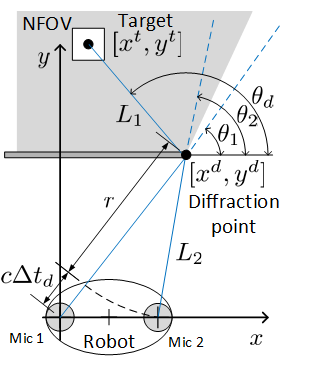
\includegraphics[width=0.5\columnwidth]{Figures/Diffraction_notation.png}
    }
    \subfigure[Magnitude with different orientation angles \cite{medwin1981shadowing}]{
        \centering
        \label{fig:diffraction2}
        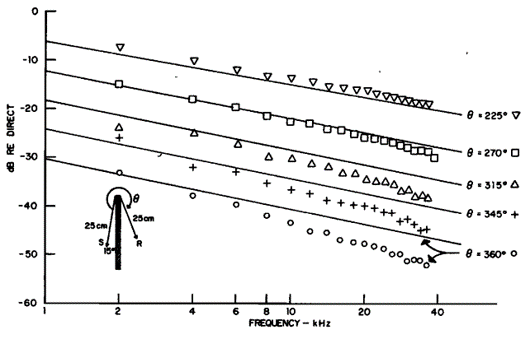
\includegraphics[width=0.8\columnwidth]{Figures/diffraction.png}
    }
    \caption{\footnotesize {Estimation of sound direction from diffraction signals} }
    \label{fig:diffraction}
\end{figure}
%%%%%%%%%%%%%%%% end figure %%%%%%%%%%%%%%%%%%%
\subsection{Estimation of Sound Direction from Diffraction Signals} Figure~\ref{fig:diffraction1} shows the notations used for target estimation from diffraction signals in the scenario introduced in the last subsection.  Since the diffraction signal microphones 1 and 2 receive is originated from the LOS location at which the sound diffracts, the proposed approach starts target estimation from diffraction signals with the selection of diffraction point from all candidates, which are corners of all structures.  The measured quantity used for the selection is the \gls{tdoa}, $\Delta t_d = t_{d2} - t_{d1}$, where $t_{d1}$ and $t_{d2}$ are the \glspl{toa} at Microphones 1 and 2 respectively.  The diffraction point can be easily found from candidates as it satisfies the following equation:  
\begin{equation}\label{eq:TDOA1}
\bs{x^d}^2 + \bs{y^d}^2 = \bs{c \Delta t_d + r}^2.  
\end{equation}
where $\bl{x^d, y^d}$ is the location of a candidate diffraction point, $c$ is the speed of sound and $r$ is a shorter distance between a microphone and the candidate diffraction point.  
With the diffraction point identified, the proposed approach further identifies the direction of the sound target from the diffraction point by analyzing the magnitudes of diffraction and reflection signals $M_i^d\bs{\omega}$ and $M_i^r\bs{\omega}$.  The loss of high-frequency signal components is assumed to be less with a microphone closer to \gls{los}, microphone 2 in this case, as there is no loss with a microphone in \gls{los} of the sound target. Medwin~\cite{medwin1981shadowing} proved the validity of this assumption over a quarter of a century ago, as shown in Fig.~\ref{fig:diffraction2}.  The magnitude of diffraction sound drops when the ``degree of \gls{nlos}'' represented by the orientation angle is increased. This makes the proposed approach define the diffraction loss as
\begin{equation}\label{eq:loss}
L_i = \int \bl{M_i^r\bs{\omega} - M_i^d\bs{\omega}} {\rm d} \omega \geq 0, \forall i \in \bm{1,2}  
\end{equation}
and associate it with the degree of \gls{nlos}.  The work of Medwin also proved that the diffraction loss is approximately proportional to the degree of \gls{nlos}.  The sound direction from the diffraction point is given by
\begin{equation}\label{eq:direction_diffraction}
\theta_d = \theta_1 + \frac{\theta_2 - \theta_1}{L_1 - L_2} L_1.   
\end{equation}

\subsection{Estimation of Sound Direction from Reflection Signals} Figure~\ref{fig:reflection} shows the proposed approach for estimation of sound direction from reflection signals.  Reflection makes the sound propagation and the subsequent target estimation complicated, but if the wall is smooth and yields specular reflection, the sound direction can be estimated easily by introducing a virtual target \cite{pulkki1997}, which is located symmetrically to the real target relative to the wall of reflection. Let the position of the virtual target be $\bl{\hat x^t, \hat y^2}$.  The measured \gls{tdoa} can be associated with the position of the virtual target as\\
%%%%%%%%%%% begin figure %%%%%%%%%%%%%%%%%%%
\begin{figure}[h]
    {\centering
        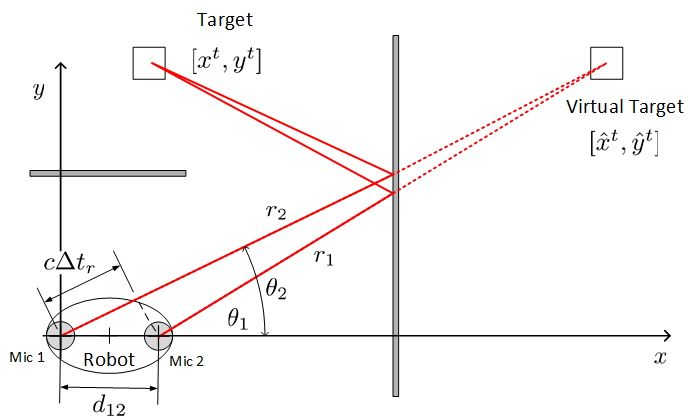
\includegraphics[width=0.9\columnwidth]{Figures/Reflection_notation.png}
    }
    \caption{\footnotesize {Estimation of sound direction from reflection signals by proposed approach} }
    \label{fig:reflection}
\end{figure}
%%%%%%%%%%%%%%%% end figure %%%%%%%%%%%%%%%%%%%
\begin{multline}\label{eq:reflection}
\left\{
\begin{array}{ll}
c\Delta t_r = \Delta r_{12}=\norm{r_1-r_2}\\
\norm{r_1}\sin{\theta_1}=\norm{r_2}\sin{\theta_2}\\
\norm{r_2}\cos{\theta_2}-\norm{r_1}\cos{\theta_1}=d_{12}
\end{array},
\right.
\end{multline}
where $d_{12}$, $\{r_1,r_2\}$ are the distance between Microphones 1 and 2 and vectors from sensor to the virtual sound source, respectively. Derivation attempted as a preliminary study for this project yields the relationship as a \gls{tdoa} curve expressing $r_1$ as a function of $\theta_1$
\begin{equation}\label{eq:estimation_reflection}
\norm{r_1(\theta_1)}=\frac{-d_{12}^2+\Delta r_{12}^2}{2(\Delta r_{12}+d_{12}\cos(\theta_1))}
\end{equation}
Further mathematical manipulation shows that this equation asymptotically yields the sound direction as 
\begin{equation}\label{eq:dirction_reflection}
\frac{\theta_2+\theta_1}{2} = \lim_{\norm{r_1} \rightarrow \infty} \tan^{-1} \frac{\hat y^t}{\hat x^t}= \cos^{-1} \frac{c \Delta t_d}{d_{12}}.   
\end{equation}
%%%%%%%%%%% begin figure %%%%%%%%%%%%%%%%%%%
%\begin{figure}[h]
%    \centering
%        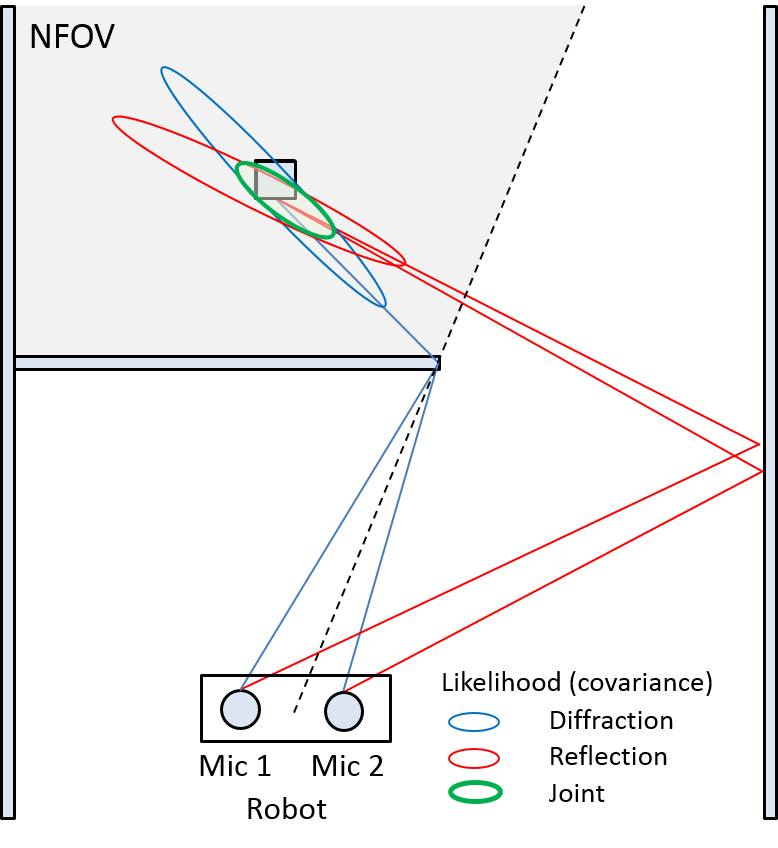
\includegraphics[width=0.30\textwidth]{Figures/data_fusion.png}
%    \caption{\footnotesize {Construction of joint observation likelihood through data fusion} }
%    \label{fig:data_fusion}
%\end{figure}

\begin{figure}[thpb]
  \centering
%  \framebox{
  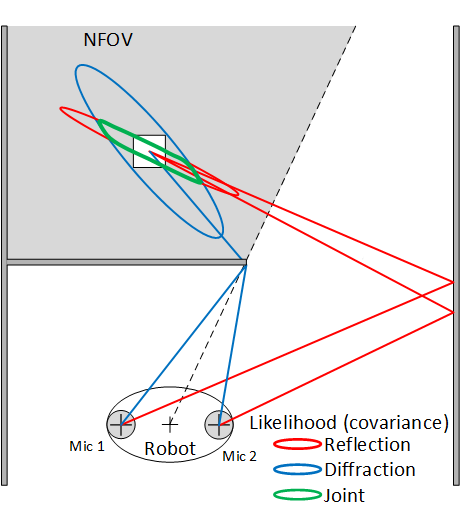
\includegraphics[width=0.7\columnwidth]{Figures/Joint_likelihood.png} %}
  \caption{Construction of joint observation likelihood through data fusion}
  \label{fig:data_fusion}
\end{figure}
%%%%%%%%%%%%%%%% end figure %%%%%%%%%%%%%%%%%%%
\subsection{ Construction of Joint Observation Likelihood through Data Fusion} 
While the sound can be better identified in direction rather than distance, it is also possible to make an estimate as to how far away the sound target is.  The proposed approach estimates  the positions by utilizing any available information including the magnitude, sound patterns, or sound features stored in a knowledge base and constructs an observation likelihood for each of the diffraction and reflection signals by modeling uncertainties.  For the $j$-th pair of microphones, the diffraction and reflection likelihoods are then combined to create an auditory joint observation likelihood via the canonical data fusion formula: 
\begin{multline}\label{eq:joint_auditory}
\lia{\Vxbp{k}{t}|\ptVzbp{s}{k}{t},\mVxbp{k}{s},\mVmb{k}} = \\ \lid{\Vxbp{k}{t}|\ptVzbp{s}{k}{t},\mVxbp{k}{s},\mVmb{k}} \lir{\Vxbp{k}{t}|\ptVzbp{s}{k}{t},\mVxbp{k}{s},\mVmb{k}} 
\end{multline}
where $\lid{\cdot}$ and $\lir{\cdot}$ are the diffraction and reflection observation likelihood.  
Figure~\ref{fig:data_fusion} illustrates the diffraction and reflection observation likelihoods as well as the joint observation likelihood where the observation likelihood is represented by an ellipsoid indicating a probability distribution with a covariance.  The diffraction and reflection likelihoods are shown to have high eccentricity due to more accuracy in direction than in distance.  Since the difference of the diffraction and reflection likelihoods in orientation may not be significant, the resulting auditory joint likelihood is also given by an ellipsoid with high eccentricity. However, the proposed approach, utilizing the diffraction and reflection physics of sound, could estimate the location of the sound target.  
%=================================================================


%\begin{table}[h]
%\caption{An Example of a Table}
%\label{table_example}
%\begin{center}
%\begin{tabular}{|c||c|}
%\hline
%One & Two\\
%\hline
%Three & Four\\
%\hline
%\end{tabular}
%\end{center}
%\end{table}


%   \begin{figure}[thpb]
%      \centering
%      \framebox{\parbox{3in}{We suggest that you use a text box to insert a graphic (which is ideally a 300 dpi TIFF or EPS file, with all fonts embedded) because, in a document, this method is somewhat more stable than directly inserting a picture.
%}}
%      %\includegraphics[scale=1.0]{figurefile}
%      \caption{Inductance of oscillation winding on amorphous
%       magnetic core versus DC bias magnetic field}
%      \label{figurelabel}
%   \end{figure}

\section{Numerical Analysis}
The preliminary simulation experiments demonstrate the validity of the proposed approach. The experiments were setup with the parameters in Table~\ref{tab:sim_parameter}.
Figure~\ref{fig:localization} shows an example of localization. The dashed line, square, circles and red cross are the reflective wall, target, microphone sensors and target estimation, respectably. As shown in the figure, diffraction and reflection observation likelihood construct the green lined joint likelihood to estimate the target location under NFOV condition.
Based on the initial simulation, the parametric study was performed to measure the sensitivity of estimation based on the sensor distance $d_{12}$ in a range of 1~cm to 50~cm. The sensor position was also varied at three different locations. Figure~\ref{fig:mic_param} shows the certainty of the target estimation as KL-Divergence at different sensor location with increasing $d_{12}$. As shown in the figure, increasing the distance between the microphone leads to a better estimate of the target. This is expected because increasing $d_{12}$ will increase the time of arrival difference, resulting in better angle estimation. However, increasing the sensor position in y-direction lead to the reduction in KL-divergence.



\begin{table}[h]
    \centering \caption{Dimensions and parameters for the simulation}
    \label{tab:sim_parameter}
    \begin{tabular}{r|r}
        \hline\noalign{\smallskip}
        Parameter & Value \\
         \noalign{\smallskip}\hline\noalign{\smallskip}
         $x^t$ & $[0.5m, 1.5m]$ \\
         $[x^d, y^d]$ & $[1m, 1m]$ \\
         $x_{wall}$ & $2m$\\
         $x_s$ & $[0.6m,0.3m]$\\
        \noalign{\smallskip}\hline\noalign{\smallskip}
     \end{tabular}
\end{table}

\begin{figure}[thpb]
  \centering
%  \framebox{
  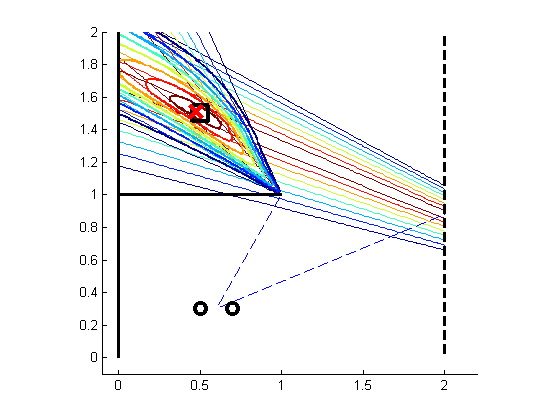
\includegraphics[width=\columnwidth]{Figures/estimation.png} %}
  \caption{Target estimation}
  \label{fig:localization}
\end{figure}

\begin{figure}[thpb]
    \centering
    %  \framebox{
    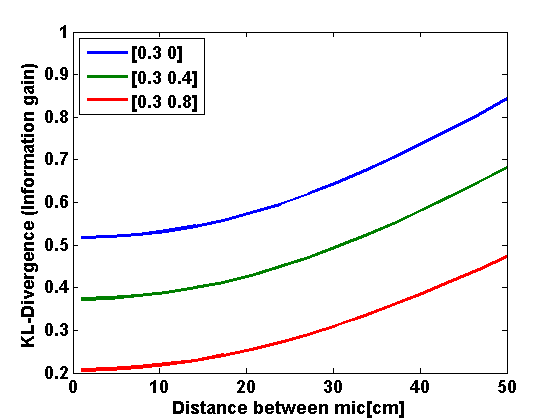
\includegraphics[width=0.7\columnwidth]{Figures/sensor_param.png} %}
    \caption{$d_{12}$ variation effect in certainty}
    \label{fig:mic_param}
\end{figure}

Figure~\ref{fig:exp_photo} show the experimental testing environment. As shown in the figure, the pink cylinder on top is the omni-directional target sound source, and separator wall and microphone array shown below. The sound insulator was installed at the top and the bottom of the environment to mitigate additional reflection and minimize reverberation. A removable smooth reflective wall was used for introducing the reflection. The experiments included microphones in a circular pattern as shown in Fig.~\ref{fig:dimension} with dimensions in Table~\ref{tab:experimental_param}.
\begin{figure}[thpb]
    \centering
    %  \framebox{
    \subfigure[Setup]{
    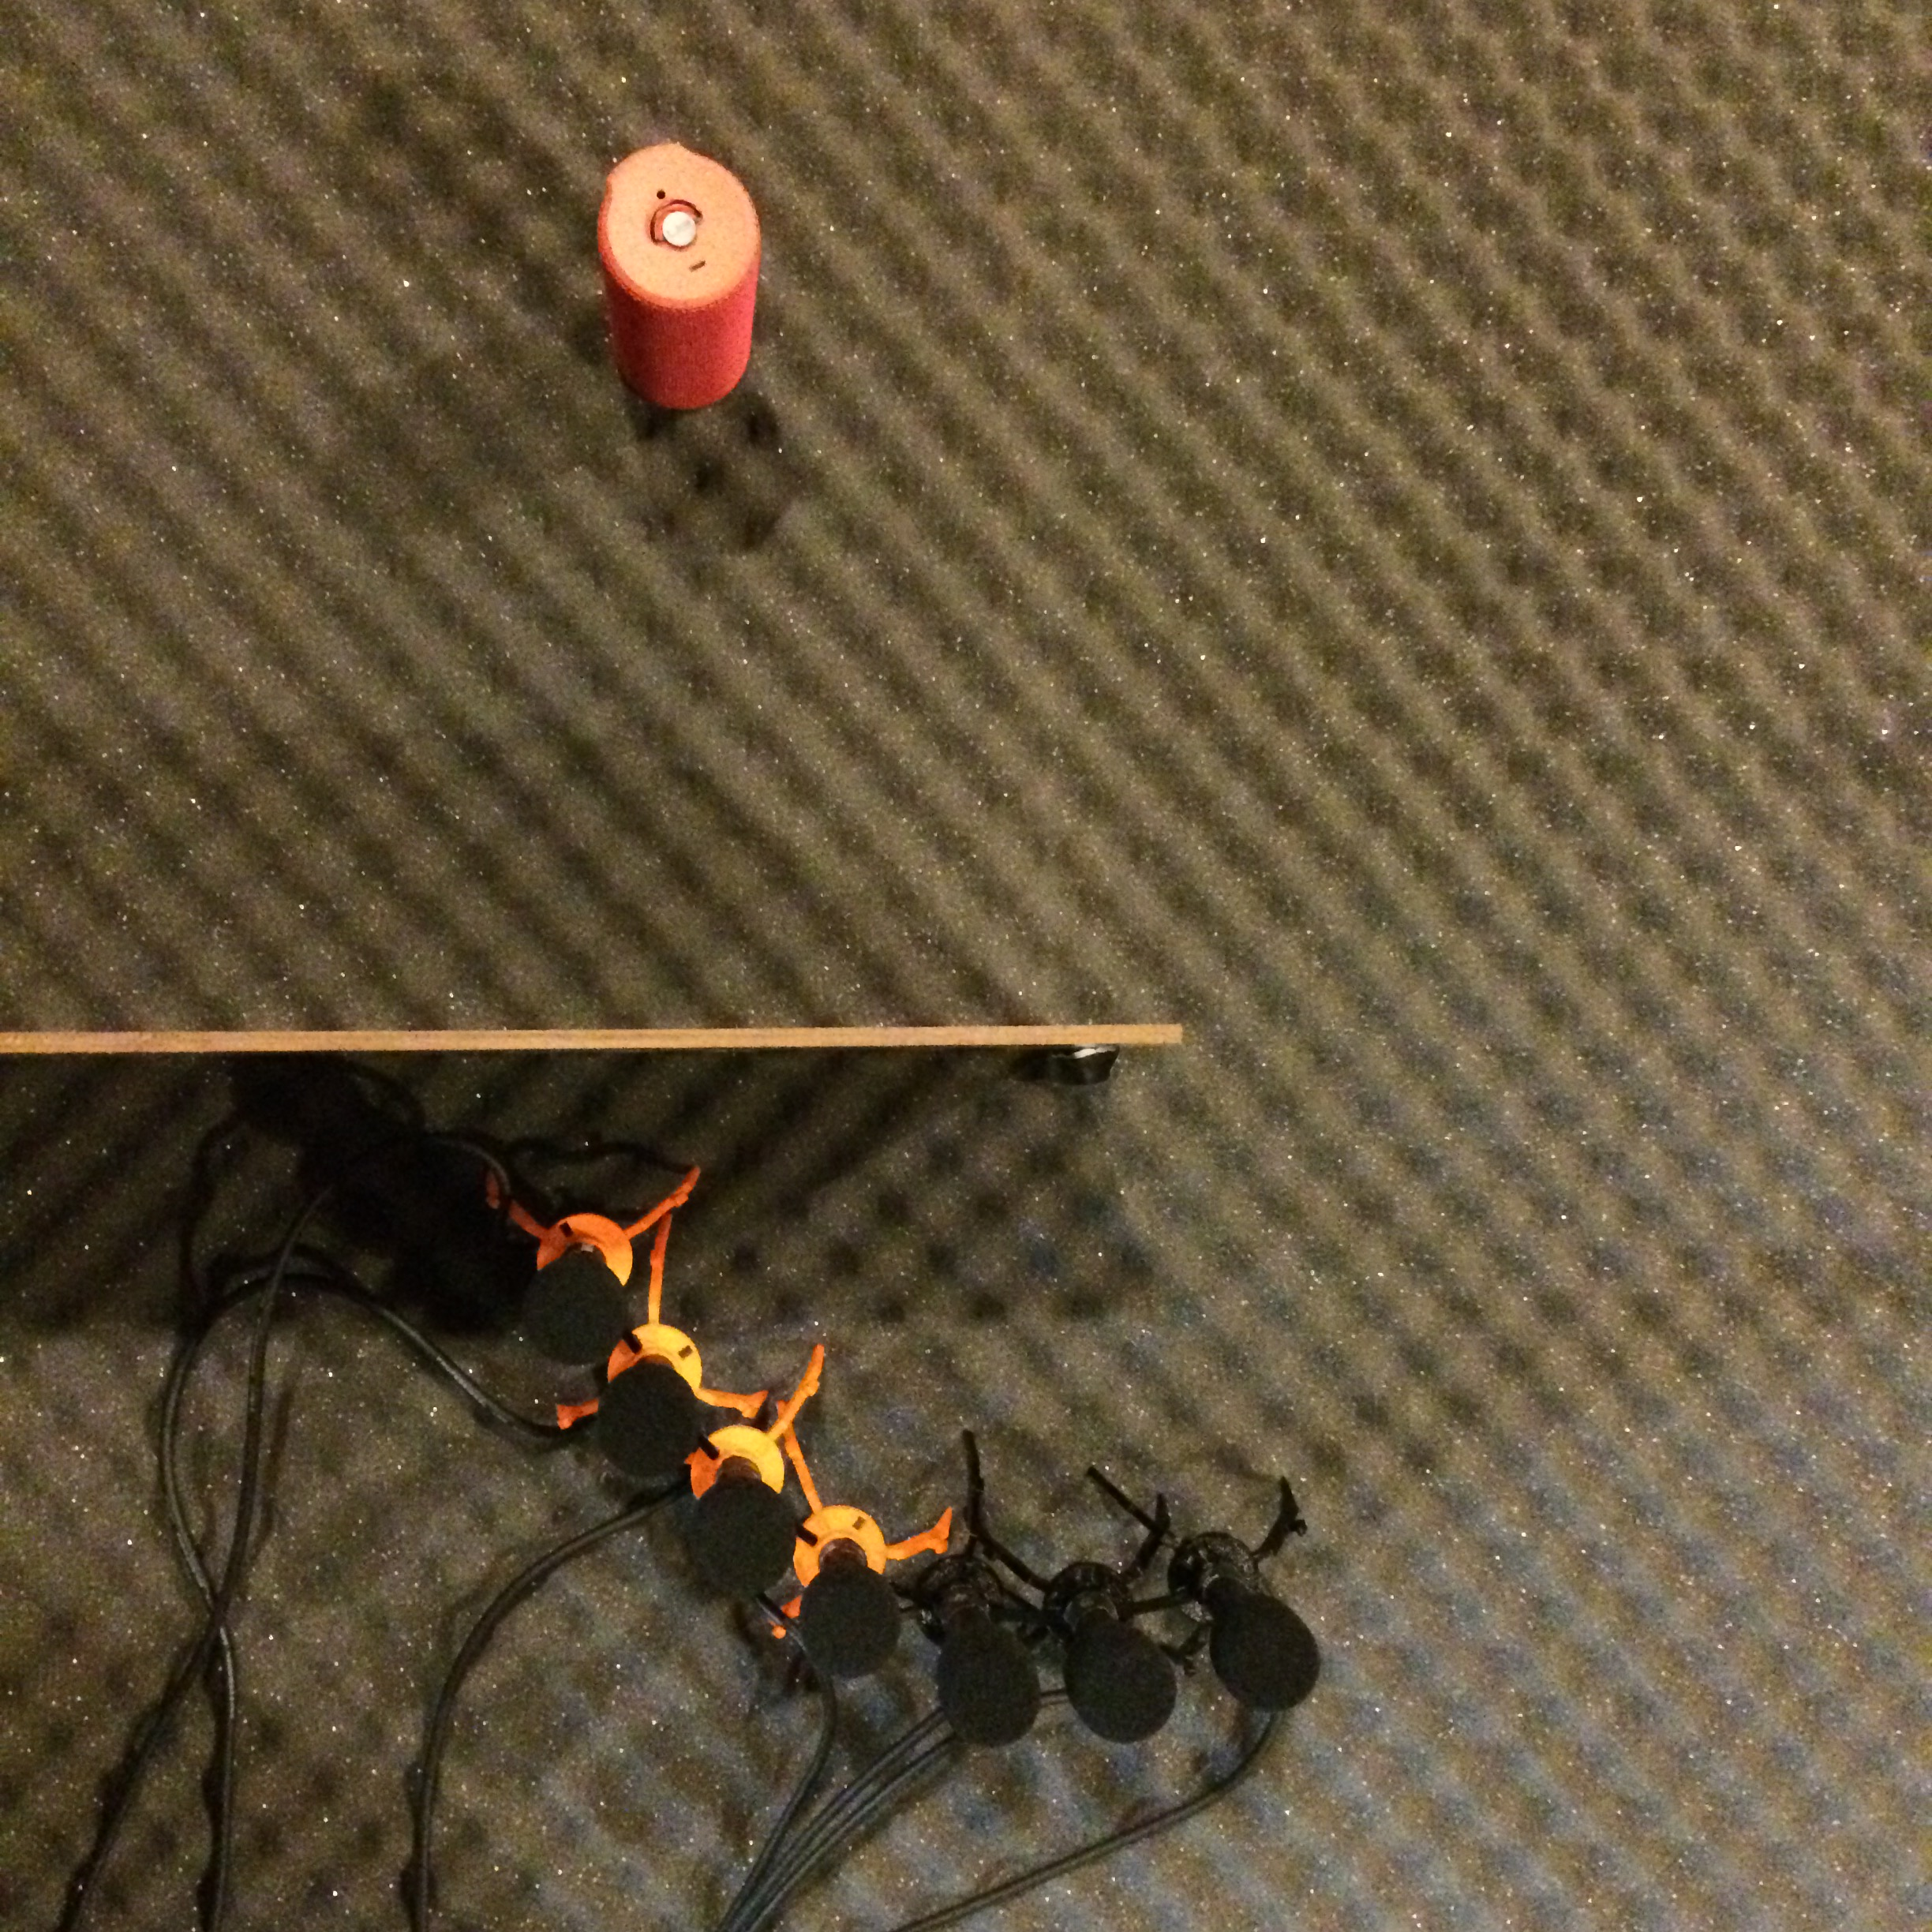
\includegraphics[width=0.6\columnwidth]{Figures/experiment.jpg} %}
	\label{fig:exp_photo}}
    \subfigure[Environemnt parameters]{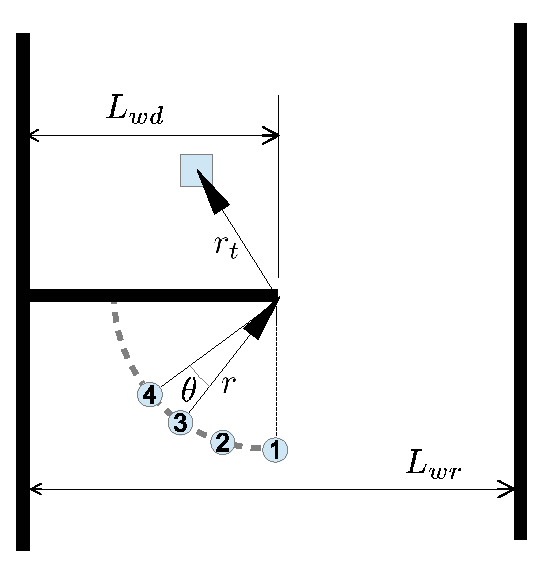
\includegraphics[width = 0.6\columnwidth]{Figures/exp_dim.eps}
    \label{fig:dimension}}    
    \caption{Experimental environment}
    \label{fig:exp_total}
\end{figure}

\begin{table}[h]
    \centering \caption{Dimensions and parameters for the experiments}
    \label{tab:experimental_param}
    \begin{tabular}{r|r}
        \hline\noalign{\smallskip}
        Parameter & Value \\
         \noalign{\smallskip}\hline\noalign{\smallskip}
         $L_{wd}$ & $62\text{cm}$ \\
         $r_t$ & $[-20\text{cm}, 25\text{cm}]$ \\
         $\norm{r}$ & $35 \text{cm}$\\
         $\theta$ & $15^\circ$\\
         $L_{wr}$ & $112\text{cm}$\\
        \noalign{\smallskip}\hline\noalign{\smallskip}
     \end{tabular}
\end{table}

Figure~\ref{fig:signal} depicts incoming sound to the microphone array without the reflection wall. The figure consist of a reference microphone at the target and the microphone array signal. As shown in the figure, the diffraction loss increased when angle of diffraction is enlarged from mic-1 to mic-4. The region A in particular displays first arrival diffraction signal. The diffraction loss is more clearly identified in the frequency domain depicted in Fig.~\ref{fig:EnergyAngle}. 

\begin{figure}[thpb]
    {\centering
    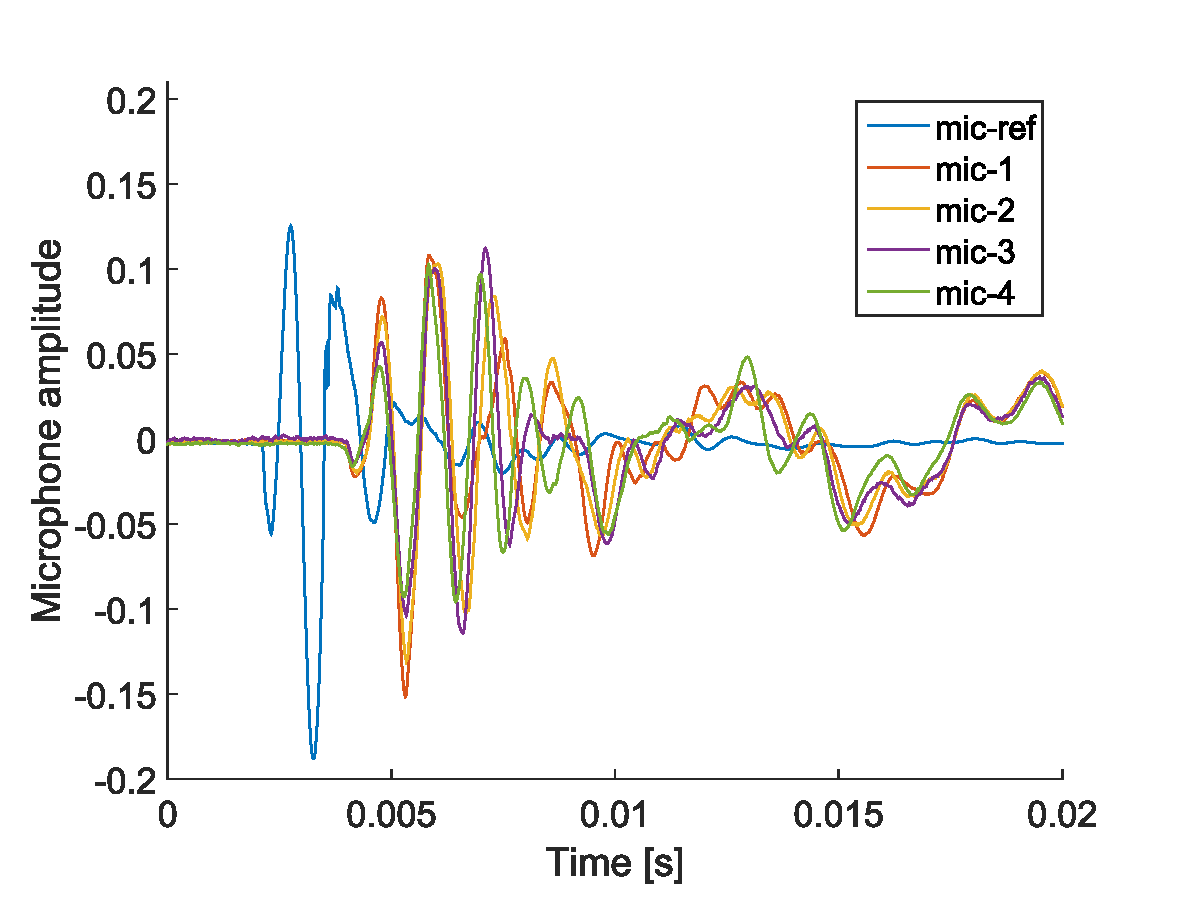
\includegraphics[width=0.8\columnwidth]{Figures/diffraction_signal.eps}
	}
    \caption{Reference mic signal at the target and signal of mic array}\label{fig:signal}
\end{figure}

\begin{figure}[thpb]
    {\centering
    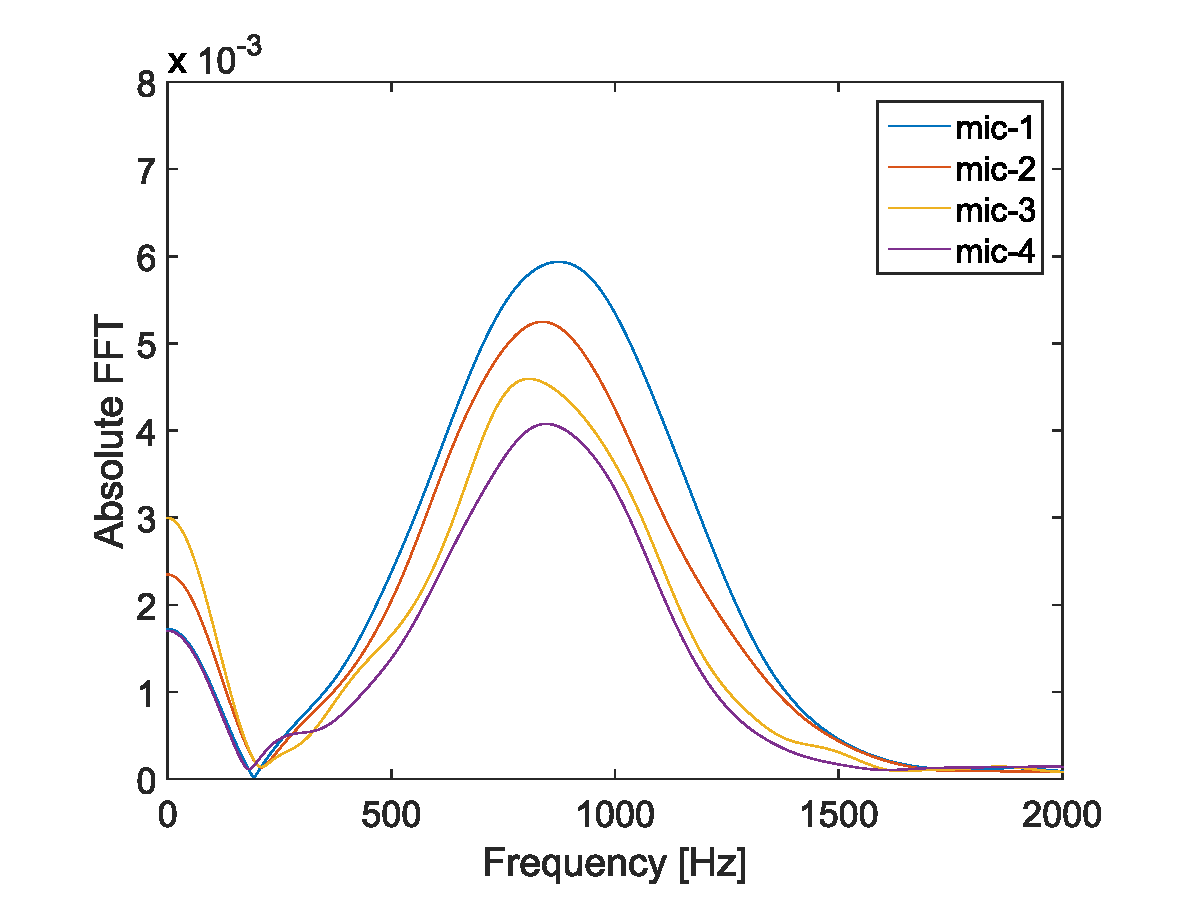
\includegraphics[width = 0.8\columnwidth]{Figures/frequency_first_peaks.eps}
    }    
    \caption{Magnitude with different orientation angles}\label{fig:EnergyAngle}
\end{figure}

Figure~\ref{fig:dr_compare} is a comparison of mic-2 signals with and without the reflection wall. The figure clearly shows the effect of the wall between those two cases where region A only contains diffraction, and region B contains mixture of diffraction and reflection. The duration of region A was measured to be less than 5\% error from the actual distance measurements.

\begin{figure}[thpb]
    {\centering
    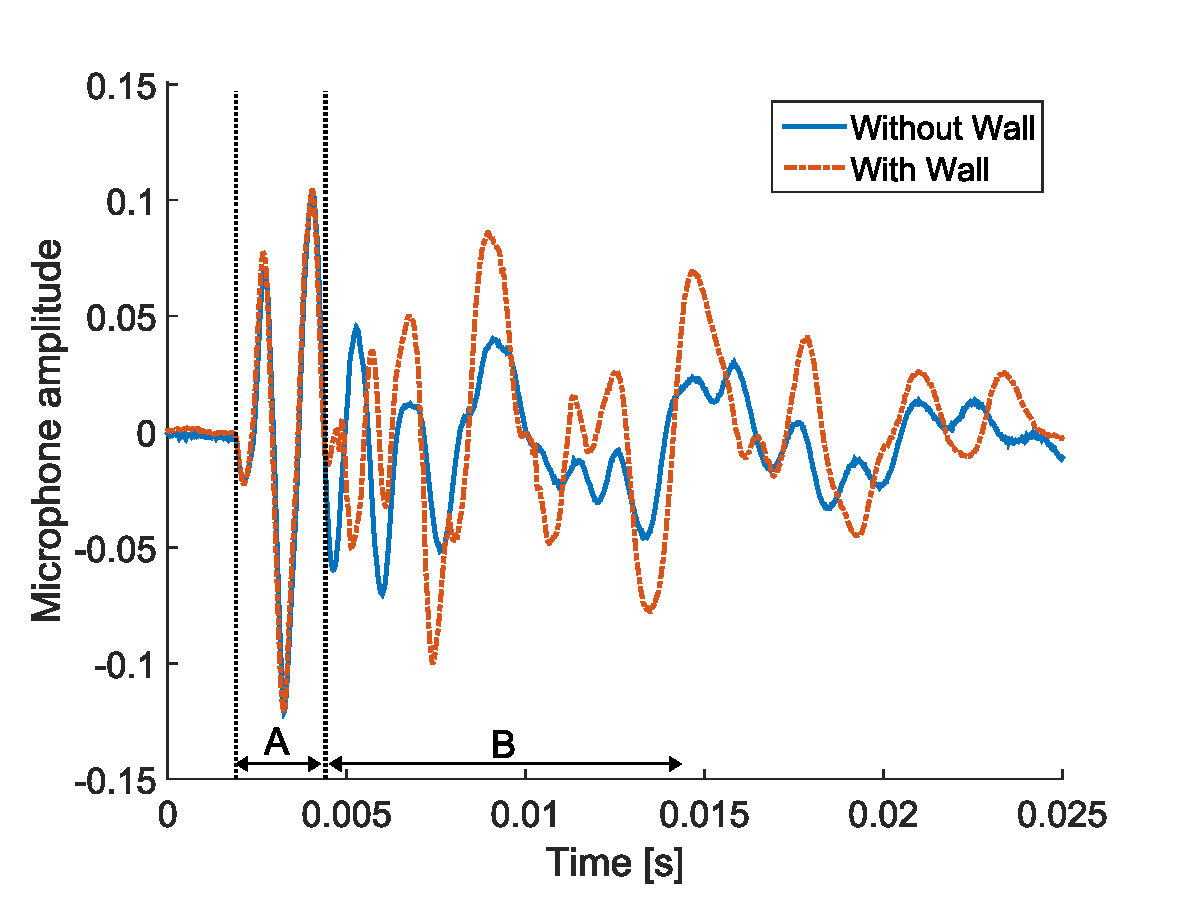
\includegraphics[width = 0.8\columnwidth]{Figures/signal_withwithout_wall.eps}
    }
    \caption{Signal with and without the reflective wall}
    \label{fig:dr_compare}    
\end{figure}

\section{CONCLUSIONS}
This paper demonstrated the target estimation capability of a new acoustic approach in \gls{nfov} using sound wave physical properties, reflection, and diffraction. This approach using sound source reflection and diffraction signal to construct two distinct observation likelihoods from the target sound. The joint acoustic observation likelihood can then be used to estimate the target location. This process was formulated mathematically with two-dimensional assumptions. The proposed approach was tested and parametrically studied under different conditions in the simulation. Finally, an experimental environment was constructed for further validation.

Future work consists of extending the application to an indoor environment. This includes the incorporation of an actual mobile target estimation using a mobile robot equipped1 with a microphone array.
%\addtolength{\textheight}{-10cm}
   % This command serves to balance the column lengths
                                  % on the last page of the document manually. It shortens
                                  % the textheight of the last page by a suitable amount.
                                  % This command does not take effect until the next page
                                  % so it should come on the page before the last. Make
                                  % sure that you do not shorten the textheight too much.
                                  
\bibliographystyle{ieeetran}            
\bibliography{References/cite_cur}   % name your BibTeX data base
%%%%%%%%%%%%%%%%%%%%%%%%%%%%%%%%%%%%%%%%%%%%%%%%%%%%%%%%%%%%%%%%%%%%%%%%%%%%%%%%
%%%%%%%%%%%%%%%%%%%%%%%%%%%%%%%%%%%%%%%%%%%%%%%%%%%%%%%%%%%%%%%%%%%%%%%%%%%%%%%%
%%%%%%%%%%%%%%%%%%%%%%%%%%%%%%%%%%%%%%%%%%%%%%%%%%%%%%%%%%%%%%%%%%%%%%%%%%%%%%%%
%\section*{APPENDIX}
%Appendixes should appear before the acknowledgment.
\section*{ACKNOWLEDGMENT}
The authors wish to acknowledge the support of the research team member, Hanxing Liu, for his efforts and very productive work and development of the experimental system and data acquisition.
%%%%%%%%%%%%%%%%%%%%%%%%%%%%%%%%%%%%%%%%%%%%%%%%%%%%%%%%%%%%%%%%%%%%%%%%%%%%%%%%
\end{document}